\section{Durchführung}
Der Versuchsaufbau besteht aus einer Steckplatine, an die ein Oszilloskop und ein Funktionsgenerator angeschlossen werden können, sowie verschiedenen Elektronikbauteilen. Der exakte Aufbau der einzelnen Versuchsteile wird in \autoref{sec:Schaltungen} beschrieben.

%überall Werte für Widerstände und Kondensatoren ergänzen?

%\subsection{Invertierender Linearverstärker}
\textbf{Invertierender Linearverstärker} \newline
Zunächst wird ein wie in \autoref{fig:InvLinear} abgebildeter invertierender gegengekoppelter Linearverstärker aufgebaut. Die Ausgangsspannung des Verstärkers wird für drei Verstärkungsgrade, das heißt für drei Widerstandsverhältnisse, in Abhängigkeit der Frequenz gemessen. %(Die Verstärkung fällt mit steigender Frequenz bei sinusförmigen Eingangssignalen ab.) 
Dabei wird ebenfalls die Phase zwischen Ein- und Ausgangssignal gemessen.
Die verwendeten Widerstände und die somit resultierenden Verstärkungen stehen in \autoref{tab:Verstaerkungen}.
\begin{table}
\centering
\begin{tabular}{lll}
    \hline
    $R_1$ & $R_2$ & $V$ \\
    \hline
    $\SI{1}{\kilo\ohm}$ & $\SI{100}{\kilo\ohm}$ & 100\\
    $\SI{10}{\kilo\ohm}$ & $\SI{100}{\kilo\ohm}$ & 10\\
    $\SI{100}{\ohm}$ & $\SI{100}{\kilo\ohm}$ & 1000\\
    \hline
\end{tabular}
\caption{Die verwendeten Widerstände und resultierende Verstärkungen.}
\label{tab:Verstaerkungen}
\end{table}


%\subsection{Umkehr-Integrator}
%\label{sec:Umkehr}
\textbf{Umkehr-Integrator} \newline
Anschließend wird der in \autoref{fig:UmkehrInt} gezeigte Umkehr-Integrator aufgebaut. Dabei werden ein Widerstand mit dem Wert $R = \SI{10}{\kilo\ohm}$ und ein Kondensator mit Kapazität $C = \SI{100}{\nano\farad}$ verwendet.
Das Eingangssignal ist sinusförmig und in Abhängigkeit von dessen Frequenz wird die Amplitude der Ein- und Ausgangsspannung gemessen.
%Es wird die Proportionalität zwischen der Ausgangsspannung und dem Kehrwert der Frequenz für ein sinusförmiges Eingangssignal gemessen und so überprüft, dass die gewählte Zeitkonstante sinnvoll ist.
Es werden ein Bildschirmfoto sowie die Daten der Ein- und Ausgangssignale am Oszilloskop für sinusförmige, dreieckförmige und rechteckförmige Eingangssignale gespeichert.



%\subsection{Invertierender Differenzierer}
\textbf{Umkehr-Differenzierer} \newline
In diesem Versuchsteil wird die Umkehr-Differenzierer-Schaltung aus \autoref{fig:InvDiff} aufgebaut und dieselben Schritte wie für den Integrator werden wiederholt. Dabei beträgt der Wert des Widerstands $R = \SI{100}{\kilo\ohm}$ und die Kapazität des Kondensators $C = \SI{22}{\nano\farad}$.
%die Schritte aus \autoref{sec:Umkehr} wiederholt.



%\subsection{Nicht-invertierende Schmitt-Trigger}
%\label{sec:Schmitt}
\textbf{Schmitt-Trigger} \newline
Um eine Messung an einem Schmitt-Trigger durchzuführen, wird die Schaltung in \autoref{fig:Schmitt} aufgebaut.
Die Werte der verwendeten Widerstände sind $R_1 = \SI{1}{\kilo\ohm}$ und $R_2 = \SI{100}{\kilo\ohm}$.
Es wird ein sinusförmiges Eingangssignal angelegt und die Eingangsamplitude wird von ihrem minimal einstellbaren Wert in kleinen Schritten erhöht.
Die Spannungsamplitude, bei der die Schaltung beginnt zu kippen, wird bestimmt.
%Alternativ: Dreieckssignal
Am Oszilloskop werden auch hierfür die Daten von Ein- und Ausgangsspannung gespeichert.
%Hysterese-Verlaufskurve ?



%\subsection{Signalgenerator}
\textbf{Signalgenerator} \newline
Im letzten Versuchsteil wird mit Hilfe von Operationsverstärkern ein Signalgenerator gebaut.
Hinter die Schmitt-Trigger-Schaltung aus dem vorherigen Versuchsteil wird ein Integrator mit Widerstand $R_3 = \SI{100}{\kilo\ohm}$ und Kapazität des Kondensators $C = \SI{1}{\micro\farad}$ geschaltet (siehe \autoref{fig:Signal}). Das Eingangssignal ist sinusförmig und das resultierende Ausgangssignal dreiecksförmig. Die Frequenz und die Amplitude der erzeugten Schwingung werden bestimmt.



%\subsection{Variierende Amplituden}
%Die Schaltung für variierende Amplituden wird wie in \autoref{fig:VarAmp} aufgebaut. Der Wert für die Kapazität ist $C = \SI{20}{\nano\farad}$. %oder 100
%Die Dämpfung/ Enddämpfung kann am Potentiometer P zwischen -1 und 1 variiert werden.
%Die \autoref{eq:SchwingAbkling} soll nachgewiesen werden.

%Für den Fall, dass $\eta < 0$ ist, wird eine gedämpfte Schwingung mit dem Oszilloskop aufgenommen. Hier muss zusätzlich eine Rechteckspannung eingespeist werden, da das System nicht von selbst schwingt.

%Für den Fall, dass $\eta > 0$ ist, wird eine charakteristische Frequenz/ Schwingungsdauer ausgemessen.

%\begin{figure}
%    \centering
%    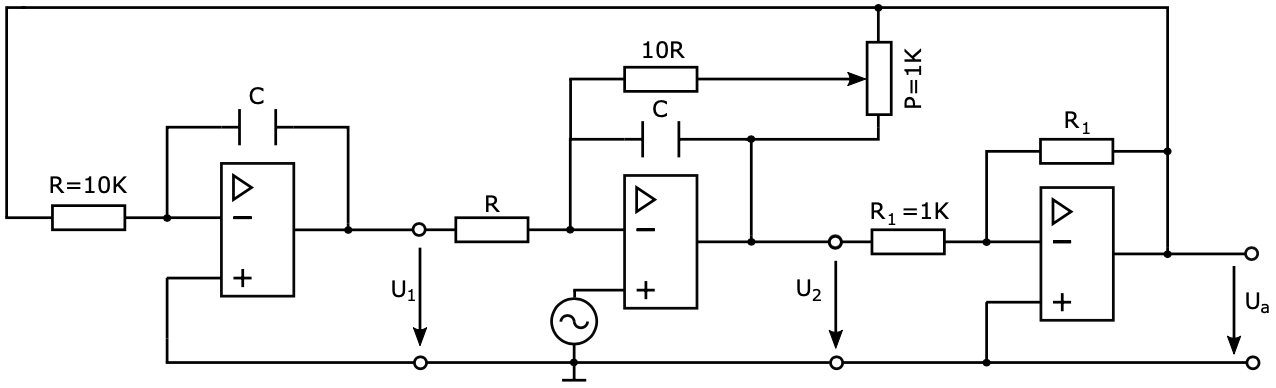
\includegraphics[width=0.7\linewidth]{./figures/6_VarAmp.png}
%    \caption{Aufbau. \cite{Anleitung}}
%    \label{fig:VarAmp}
%\end{figure}